% !TeX root = ./main.tex
\documentclass[journal]{Imperial_lab_report}

\ifCLASSINFOpdf

\else

\fi

\usepackage{cite}
\usepackage{fancyhdr}
\usepackage{lastpage}
\usepackage{amsmath,amssymb,amsfonts}
\usepackage{algorithmic}
\usepackage{textcomp}
\usepackage{xcolor}
\usepackage[euler]{textgreek}
\usepackage{graphicx}
\usepackage[numbers]{natbib}
\usepackage{hyperref}
\hypersetup{
    colorlinks=true,
    linkcolor=blue,
    filecolor=magenta,      
    urlcolor=blue,
}
\graphicspath{{imgs/}}
\urlstyle{same}

\begin{document}
%
% paper title
% Titles are generally capitalized except for words such as a, an, and, as,
% at, but, by, for, in, nor, of, on, or, the, to and up, which are usually
% not capitalized unless they are the first or last word of the title.
% Linebreaks \\ can be used within to get better formatting as desired.
% Do not put math or special symbols in the title.

\title{Advanced Electronics Project: Analogue Computer}


\author{V. Sridharbabu, A. Alonso Bizzi}% <-this % stops a space




% The paper headers
\markboth{V. Sridharbabu \& A. Alonso Bizzi}%
{Shell \MakeLowercase{\textit{et al.}}:}

\maketitle

\begin{abstract}

A car's suspension system was modelled by building an analogue computer. It was used to solve the differential equations that described the displacement of the suspension system from equilibrium as response to the surface displacement of the road. The circuit was simulated using LTSpice and was tested with different waveforms with known solutions. The output of the circuit was within the uncertainties of the theory. $\gamma$ values of 2$s^{-1}$ and 10$s^{-1}$ we used for light damping and heavy damping respectively. For the standard analogue computer, the resonant frequencies were: 1.2$\pm$0.3Hz for light damping and 0.4$\pm$0.3Hz for heavy damping. For the analogue computer with the inverted inverting differentiator, the resonant frequency for light damping was 1.3$\pm$0.6Hz. 

\end{abstract}


\section{Introduction}

\IEEEPARstart{A}{n} analogue computer\cite{manual} uses physical phenomena rather than using binary states (1s and 0s), like digital computers to perform mathematical operations. Analogue computers are able to handle continuous data which allow them to perform abstract calculations without needing complex computational algorithms or discretisation of the signal \cite{digitalvanalogue}. This project involves modelling a car suspension system and testing it under different conditions and damping ratios to model under-damped, over-damped and critically damped solutions.

The car suspension system is displaced from equilibrium when moving over rough terrain due to the surface displacements present. The severity of this motion is dictated by the springs and shock absorbers within the suspension \cite{mechanic}. By modelling the dynamics of suspension system \cite{suspensionmodel} over each wheel as a second-order linear non-homogeneous equation, a suitable model can be achieved by designing a circuit with operational amplifiers, which then can be compared to theory and the simulation to conclude on the effectiveness of this model.  

\section{Theory}

\subsection{Mathematical Model of the Suspension}

\begin{figure}[h]
    \centering
    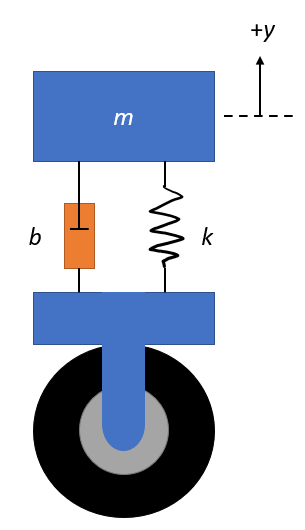
\includegraphics[width=2.5cm]{simple model.png}
    \caption{
    A simple model of a car suspension system. The mass of a quater car is connected to a spring and a shock absorber, which are attached onto a central axle that supports the wheel. The changes in the road are modelled by a force F(t) exerted upwards from the wheel which causes the car's body to displace from equilibrium (y=0).
    }
    

    \label{fig:simple model}
\end{figure}

We modelled a passive car suspension system, shown in figure Fig(1). The mass, m, above each wheel is assumed to be a quater of the car's mass.

Taking upwards as positive, the force acting on the car from the road is the input force, x(t) = F(t). The force from the spring is -ky using Hooke's Law and the damping force is modelled as  -b$\dot{y}$. The weight (mg) of the car is ignored as it is constant and doesn't contribute to the dynamics of the whole system apart from determining the equilibrium position, y=0. The sum of these force is represented by the following equation:

\begin{equation}
    x - ky - b\dot{y} = m\ddot{y}
\end{equation}

Rearranging the equation gives:
\begin{equation}
    \frac{x}{m} - \gamma \dot{y} - \omega_{0}^{2}y = \ddot{y}
\end{equation}
where $\gamma = \frac{b}{m}$ and $\omega_{0}^{2} = \frac{k}{m}$.

The functional form of the solution will depend on the damping coefficient,
\begin{equation*}\label{diff equation}
    \zeta = \frac{b}{2\sqrt{mk}} = \frac{\gamma}{2\omega_{0}}.
\end{equation*}

Critical damping: $\zeta = 1$, will yield a single full oscillation and will converge to equilibrium. Overdamping: $\zeta > 1$, will converge to equilibrium without a full oscillation. Underdamping: $\zeta < 1$, will oscillate several times before converging to equilibrium.\cite{dampedfreq}



The resonant frequency of a damped harmonic system is usually lower than the natural frequency of the system. This relationship is given by the equation:
\begin{equation}\label{resonant frequency}
    \omega = \sqrt{{\omega_0}^2 - (\frac{b}{2m})^2},
\end{equation}
%include each solution - Look at OW notes





\subsection{Circuitry - The Op-Amp}

%\subsubsection{The Op-amp}
An op-amp \cite{op-amp} is an amplifier with a high, open-loop gain, which replaces the need for multiple transistors for amplification. Op-amps are more consistent in amplifying a signal than individual transistor which would have varying current gain h$_{fe}$. Op-amps require external power in order to operate and provide gain while conserving energy. Fig(2) shows a diagram of a typical op-amp.
\begin{figure}[h]
    \centering
    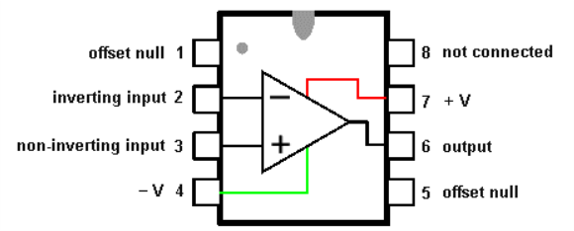
\includegraphics[width=7cm]{8pin op-amp.png}
    \caption{Top-view schematic of a typical 8-pin, dual-in-line op-amp.\cite{op-amp}}
    
    \label{fig:op-amp}
\end{figure}

%\subsubsection{Inverting}


\subsection{Problem Abstraction: Block diagram}
Fig(3) represents Eq(2) as a block diagram\cite{analoguecompanalysis}. An inversion of -$\frac{100x}{m}$ on the input is required to achieve the correct polarity from the inverting summator's output and the scaling by 100 is to ensure a large force can be represented by a practical peak to peak voltage around 5V. 

The summing of the components of Eq(2) into the summator are inverted in polarity to negate the effects of the inversion caused by the inverting summator.


%Taking the simplest case,t = 0, the body of the car has zero velocity or acceleration, so the input passes straight through the central path, giving \(y =\int \int \frac{x}{m} \,dt \,dt\) as required by Hooke's Law.



\begin{figure}[h]
    \centering
    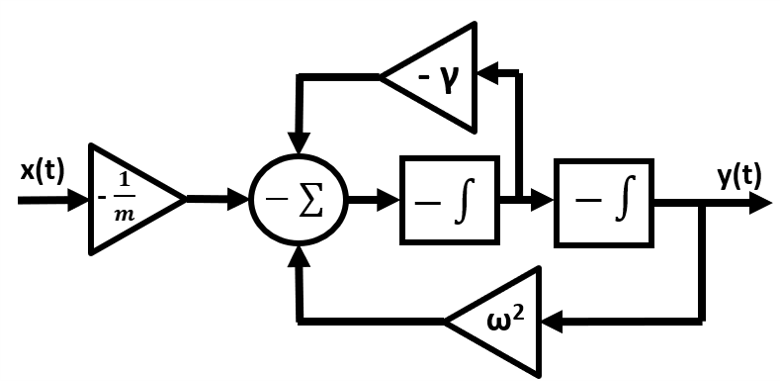
\includegraphics[width=7cm]{block diagram 2.png}
    \caption{Diagram showing abstracted circuit functionality. Where the input is split off, integrated, amplified and iteratively summated to the other inputs.}
    \label{fig:block normal}
\end{figure}
%\subsubsection{Frequency response}

\subsection{Coupling the surface displacement of the road with the suspension dynamics}
The fidelity of the analogue computer can be tested by adapting the circuitry to calculate the input force from the surface displacement of the road from x=0. Ignoring any effects from damping or wheel deformation, the forces can be calculated from the difference in displacements and velocities of x and y. This coupling gives us the equations:
\begin{equation}
    - b(\dot{y} - \dot{x}) - k(y - x) = m\ddot{y}
\end{equation}
\begin{equation}
    - \gamma(\dot{y} - \dot{x}) - \omega_0^2(y - x)  = \ddot{y}
\end{equation}

From this, the block diagram can be adapted to include $\dot{x}$ as an input to the summator, as shown in Fig(4). Thus, we need to add an inverting differentiator with an inverting amplifier of unity gain to invert the output of the differentiator.
\begin{figure}[ht]
    \centering
    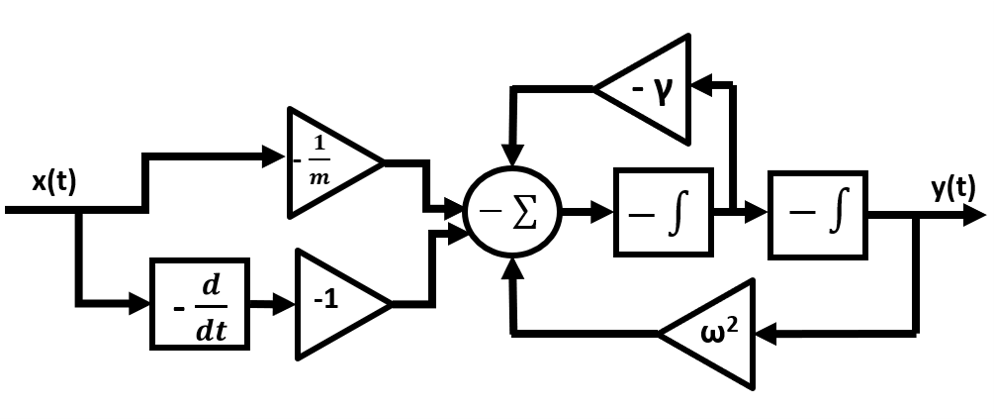
\includegraphics[width=9cm]{extension inverting differentiator.png}
    \caption{Block diagram for a circuit that considers the input as the the displacement of the road from flat.}
    \label{fig:extension}
\end{figure}

\subsection{Rectified input}
A half-wave rectifier can be used to mimic the speed bumps on the road, since these bumps are postive only. This is achieved by connecting a diode to the input signal to only allow the positive voltages.
\section{Method}
\subsection{Simulation}

To test out which components to use to give the best result the first thing we did was simulate the circuit in LTSpice. We passed through 5 different types of waves to represent the different possible input forces:

\begin{itemize}
    \item Square wave.
    Low frequencies for quasi-static testing.
    Higher frequencies for bumps and holes in the road.
    \item Sine Wave.
    Low frequencies and high frequencies
    \item Single Pulse.
    For more accurate quasi-static testing.
\end{itemize}

 The natural frequency is taken to be of a Porsche at 1.18Hz which equates to natural angular frequency of 7.41 rad$s^{-1}$. For critical damping, $\gamma$ = 14.82$s^{-1}$. The mass of the car is 1440 kg, so a quater-mass is 360kg. The capacitor values and the resistor values were adjusted during simulation on LTspice to get reliable results. 

 \begin{figure}[h]
    \centering
    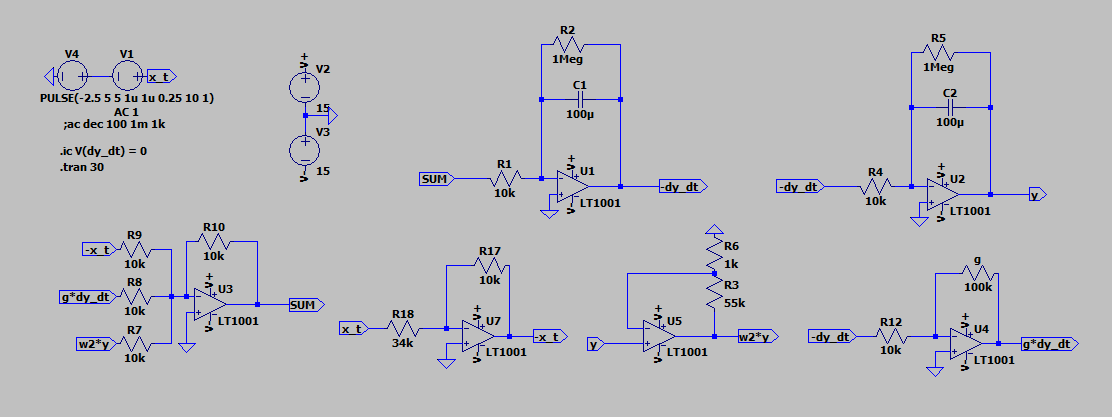
\includegraphics[scale = 0.3]{final_sim_default.PNG}
    \caption{LTSpice simulation circuit design of the standard analogue computer. Includes 1 signal generator, 1 op-amp power supply, 2 integrator circuits, 2 inverting amplifiers, 1 non-inverting amplifier and 1 inverting summator.}
 \end{figure}

During simulation, initially we decided not to use amplifiers following the integrators, but instead scale the input resistances of the summator to obtain the ideal scaling for the signals. After simualtion, it came to our realisation that the resistances were too small which was causing backflow in the circuit, as the small op-amp input resistances were not large enough for our resistance values which made the current take the path of least resistance away from the op-amp. After this realisation, we switched to the 6 op-amp design shown in Fig(5) and increased all the resistances to prevent backflow. 

As extention, we decided to introduce a differentiator to the circuit, this was to closely mimic the behaviour of the suspension system by coupling it with the surface displacement of the road.

\begin{figure}[h]
    \centering
    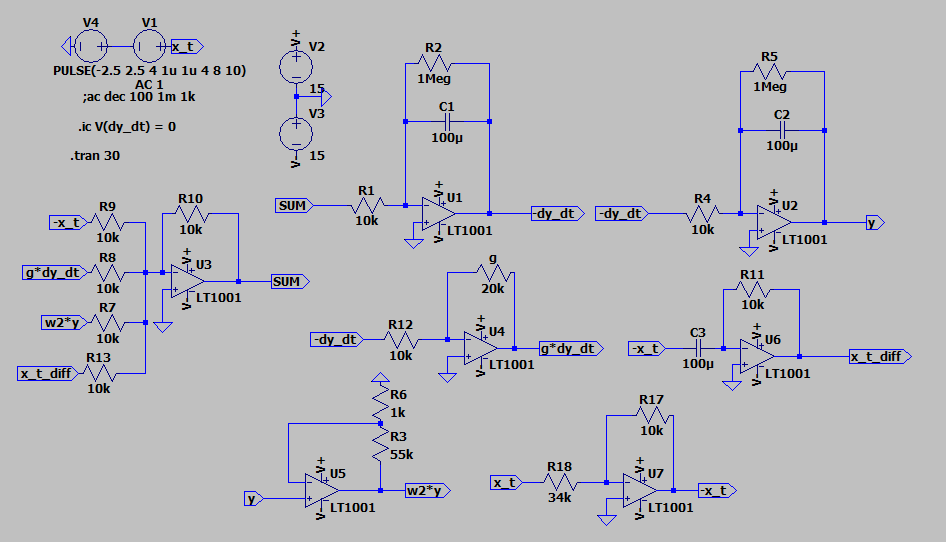
\includegraphics[scale = 0.3]{final_sim_diff.PNG}
    \caption{LTSpice simulation circuit design of the analogue computer with an inverted inverting differentiator. Includes 1 signal generator, 1 op-amp power supply, 2 integrator circuits, 2 inverting amplifiers, 1 non-inverting amplifier, 1 inverting differentiator and 1 inverting summator.}
\end{figure}

The simulation circuit with the differentiator is shown in Fig(6). The input x(t) is split into two paths, with one going into the summator through an inverted amplifier for scaling and the other through the inverting differentiator. The rest of the circuit is identical to the standard analogue computer design. This was done to make the inverting amplifier of unity gain after the differentiator redundant, as the inverting is already taken care of by the initial inverting amplifier on the input.

After testing the simulation for ideal behaviour, we built the physical circuitry for the analogue computer with the differentiator.

\begin{figure}[h]
    \centering

    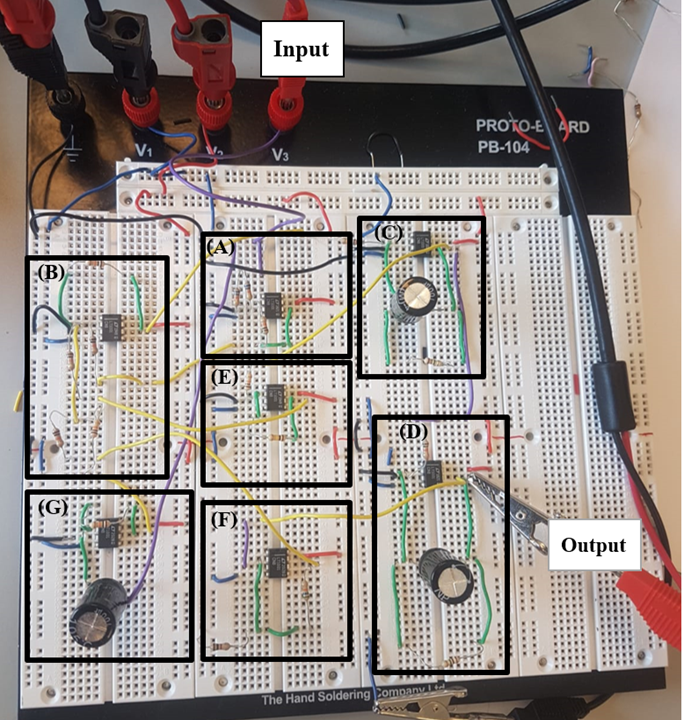
\includegraphics[scale = 0.3]{circuit.png}
    \caption{Physical circuit of the analogue computer with the inverted inverting differentiator. A - Inverting Amplifier: scaling of $100/360$, B - Inverting Summator, C - Inverting Integrator: integrates the output of the summator, D - Inverting Integrator: integrates the output of the first integrator (B), E - Inverting Amplifier: scales by $\gamma$, F - Non-Inverting Amplifier: scales by ${\omega_0}^2$, G - Inverting Differentiator: differentiates the output of A.}
\end{figure}

    \section{Results and Analysis}

    The data collected from the oscilloscope scope was quite noisy as seen in Appendix A. The retrieved data was firstly smoothed by using a moving average of 2000 datapoints and the uncertainty region of the moving average was calculated by the noise. Moving averages and fourier plots are shown in Appendix B.

    \subsection{Standard Analogue Computer}

    The standard analogue computer resulted in low voltage ranges for the output, typically around 20mV. This made the output quite noisy. The circuit was tested with various input waves: 500mHz and 2000mHz sinusoidal wave and square wave, 500mHz triangle wave and a 100mHz pulse for $\gamma$ values of 2$s^{-1}$ and 10$s^{-1}$. 

    Eventhough 10$s^{-1}$ is less than 14.82$s^{-1}$, the observed response before testing was of an overdamped solution. This is most likely due to the frequency response of the gain at low semi-low frequencies. This makes the actual scaling of the circuit difficult to estimate and the actual values for $\gamma$ and $\omega_{0}^2$ will be quite different than the theoretical values.
    
    The input 500mHz, Fig(13.b) and Fig(14.b), sinusoidal wave yieled in an output sinusoidal wave for both $\gamma$ values, in phase with the input, with about $\frac{3}{400}$ the initial magnitude.  The 2000mHz sinusoidal wave, Fig(13.a) and Fig(14.a), yieled in an output sinusoidal wave for both $\gamma$s, antiphase with the input and $\frac{3}{400}$ of the initial magnitude. The fourier analysis of the output showed frequencies around 500mHz and 2000mHz respectively for the 500mHz and the 2000mHz input sinusoidal wave.

    Similarly, the square wave of 500mHz and 2000mHz yieled in a periodic waveform in phase and antiphase respectively. The fourier analysis showed multiple frequencies superposed to give a periodic wave, the number of frequencies in effect seem to converge into a sinusoidal wave of frequency 1.93Hz as the frequency increased from 500mHz to 2000mHz with decrease in the amplitude of the resulting frequency, from a peak of 0.0231 to 0.0068. 

    The 100mHz pulse input for $\gamma = 2$$s^{-1}$ shows a clear representation of light damping. The resonant frequency of the damping is about 1.2$\pm$0.3Hz by calculating the peak of the fourier plot. Using Eq(3), we can calculate the natural frequency to be 1.4$\pm$0.7Hz using $b = {\gamma}\frac{m}{100}$.

    The 100mHz pulse input for $\gamma = 10$$s^{-1}$ shows a clear representation of heavy damping. The resonant frequency of the damping is about 0.4$\pm$0.3Hz as shown by the fourier plot. We can calculate the natural frequency to be 3$\pm$3Hz. 

    The modelled system's natural frequency is 1.18Hz. This suggests that this analogue counterpart is quite reliable for lightly damped systems that are just under critical damping, such as a common car suspension system, but less reliable for heavily damped systems.


    \subsection{Analogue Computer with an Inverted Inverting Differentiator}
    
    In order to visualise the suspension system clearly, the set-up shown is Fig(4) was used. The differentiator allowed us to view the motion of the suspension relative to the surface of the road. This circuit also boosted the amplitude of the output by ten-fold. This circuit was tested with $\gamma = 2$$s^{-1}$.

    An input 2000mHz sinusoidal wave yieled a non-sinusoidal output. The output was quite similar to a 500mHz square input on a standard analogue computer of $\gamma = 2$$s^{-1}$. The peak frequency on the fourier plot was at 0.7$\pm$0.2Hz followed by a lower peak around 2Hz, i.e. the driving frequency. The 0.7Hz is most likely caused due to damping effects of the model suspension, however frequencies of this magnitude are quite rare cases and would definitely behave drastically different in a physical scenario. 

    An input 500mHz sinusoidal wave yielded a sinusoidal wave $\frac{\pi}{2}$ out of phase. The frequency of the output was 0.5$\pm$0.2Hz, which is the same as the driving frequency of the system. This shows that at low frequencies, the lightly damped system follows smooth waveforms without undergoing any damping effects.

    An input 100mHz square wave yieled a periodic damped harmonic motion with switching polarity as seen in Fig(15.c). This was an expected outcome and shows that the motion of the suspension is reliably modelled by the analogue computer. We can also observe a vertical shift in the equilibrium point, i.e. the convergence of the damped harmonic motion, which switches from positive to negative after each subsequent change in the surface elevation of the road, Fig(8). This vertical shift represents the vertical displacement of the suspension system due to the surface displacement of the road. The fourier analysis of this graph also yieled important results; the peak of the fourier plot lies at a frequency of 1.11$\pm$0.02Hz, when taken as the resonant frequency yields a natural frequency of 1.3$\pm$0.6Hz which is close to the actual natural frequency of 1.18Hz of the system than the standard analogue computer. Fig(9) shows the same input but for $\gamma = 10$$s^{-1}$, which is overdamped.

    \begin{figure}
        \label{fig: G 2 100 Diff zoom}
        \centering
        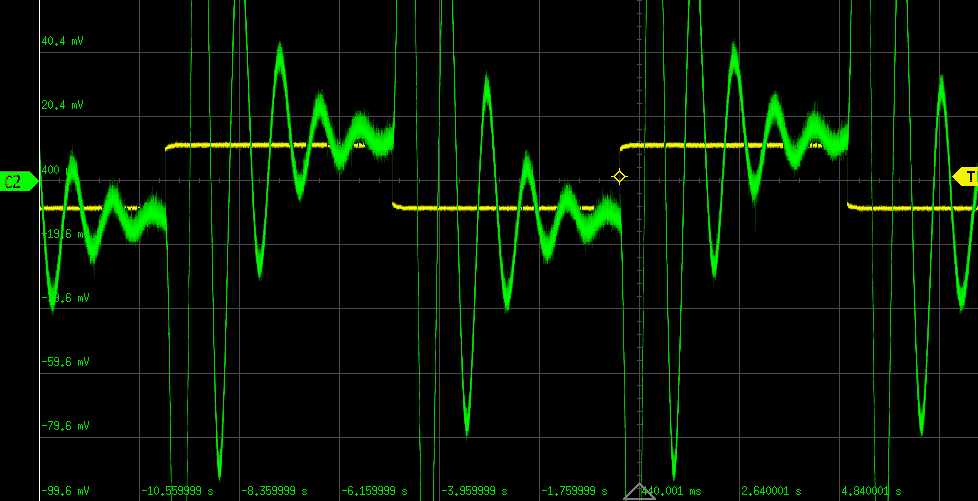
\includegraphics[scale = 0.25]{S_100_zoom.png}
        \caption{Oscilloscope screenshot of the response of the analogue computer with an inverted inverting differentiator to a 100mHz square wave input with $\gamma=2$$s^{-1}$. Scaled and positioned to show the y shift in each oscillation.}
    \end{figure}

    \begin{figure}
        \centering
        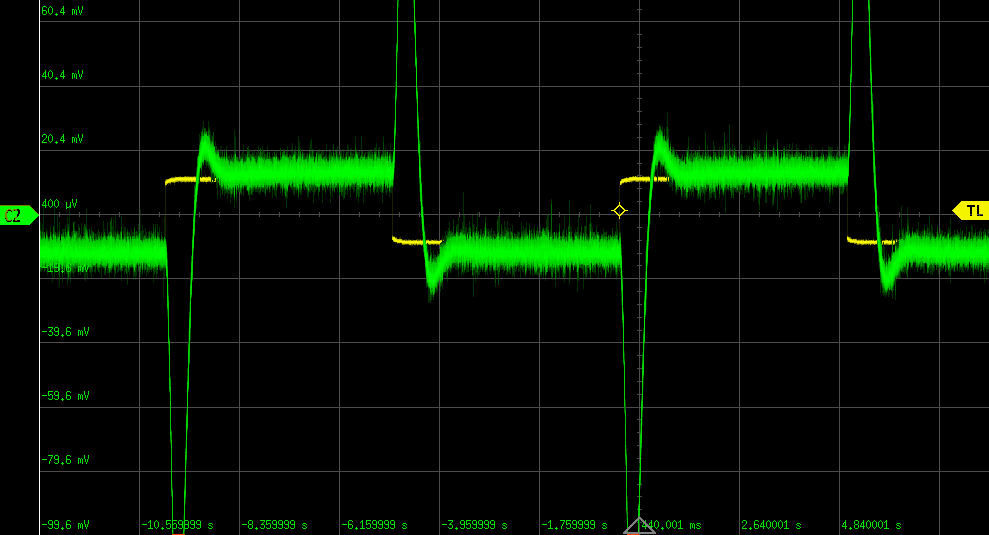
\includegraphics[scale = 0.25]{G_10_zoom.png}
        \caption{ Oscilloscope screenshot of the response of the analogue computer with an inverted inverting differentiator to a 100mHz square wave input with $\gamma=10$$s^{-1}$. Scaled and positioned to show the y shift in each oscillation.}
    \end{figure}
    An input 2000mHz square wave yieled a psuedo - sinusoidal output with a peak frequency about 2Hz, the driving frequency. Other smaller peaks were observed at 0.5Hz and 6Hz which are most likely to be harmonics of the 2Hz or due to the transient response of the system. 

    The solution with the differentiator was more reliable with reduced noise, due to the feedback of the input back into the summator - which amplified the signal.

    \subsection{Half-Wave Rectified Analogue Computer with an Inverted Inverting Differentiator}
    
    \begin{figure}[h]
        \centering
        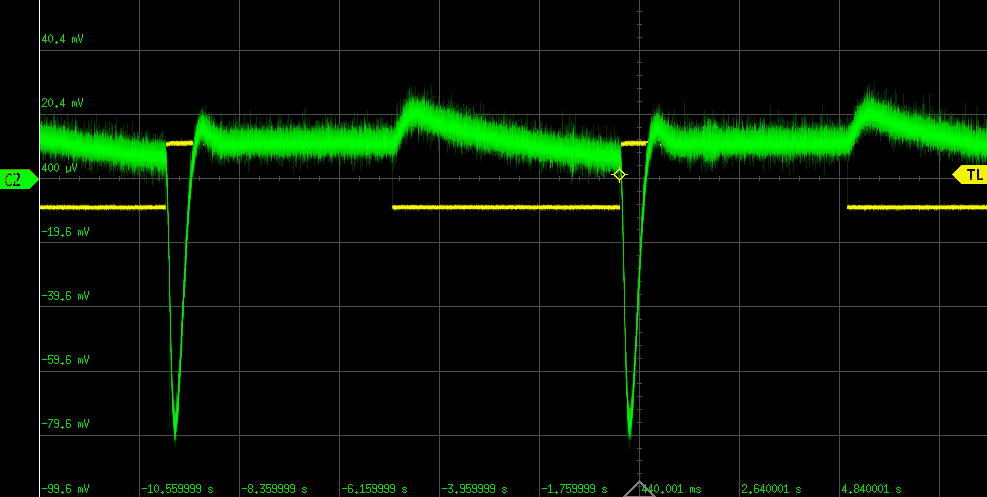
\includegraphics[scale = 0.25]{G_10_R.png}
        \caption{ Oscilloscope screenshot of the response of the half-wave rectified analogue computer with an inverted inverting differentiator to a 100mHz square wave input with $\gamma=10$$s^{-1}$. Scaled and positioned to show the y shift in each oscillation.}
    \end{figure}

    A half-wave rectifier for the input was made by attaching a diode to the input of the analogue computer.

    Fig(10) shows the response of a overdamped suspension using the half-wave rectified circuit and the dynamics of the spring as the height changes with time.
    


    \section{Conclusion}

    The standard analogue computer set-up yielded expected results for each test eventhough there was a significant amount of noise due to the small amplitudes of the output. The damping coefficients of 2$s^{-1}$ and 10$s^{-1}$, eventhough both are less than the critical damping coefficient of 14.82$s^{-1}$, 10$s^{-1}$ did produce an overdamped solution. The resonant frequency was calculated to be about 1.2$\pm$0.3Hz for light damping and 0.4$\pm$0.3Hz for heavy damping. Recalculating the natural frequencies from these values, yielded highly uncertain results for the natural frequency of 1.4$\pm$0.7Hz and 3$\pm$3Hz respectively which are quite greater than the expected 1.18Hz. The lightly damped solution is however closer to the value. This is probably due to scaling of $\gamma$ in the inverting amplifiers due to frequency response of the gain.
    
    The sinusoidal inputs for the above set-up resulted in a in-phase sinusoidal output for 500mHz and an anti-phase sinusoidal output for the 2000mHz.

    The analogue computer with the inverted inverting differentiator yielded far greater results. The output was of a greater amplitude, almost ten-times the standard output, which reduced the amount of noise in the signal. The resonant frequency was calculated for $gamma = 2$$s^{-1}$, which equated to 1.11$\pm$0.02Hz resulting in a natural frequency of 1.3$\pm$0.6Hz. This is closer to 1.18Hz than the standard set-up.

    The half-wave rectified version was quite reliable in describing the dynamics of the suspension relative to the road's surface displacement.

    Therefore, it is possible to conclude that the analogue computer did model the suspension system quite reliably in terms of the dynamics, however it did fall short on the accuracy of the system due to inaccuracies in the scaling due to the frequency response of the gain.


    \begin{appendices}
        \newpage
        \section{Noisy Data}
        \begin{figure}[h]
            
            \centering
            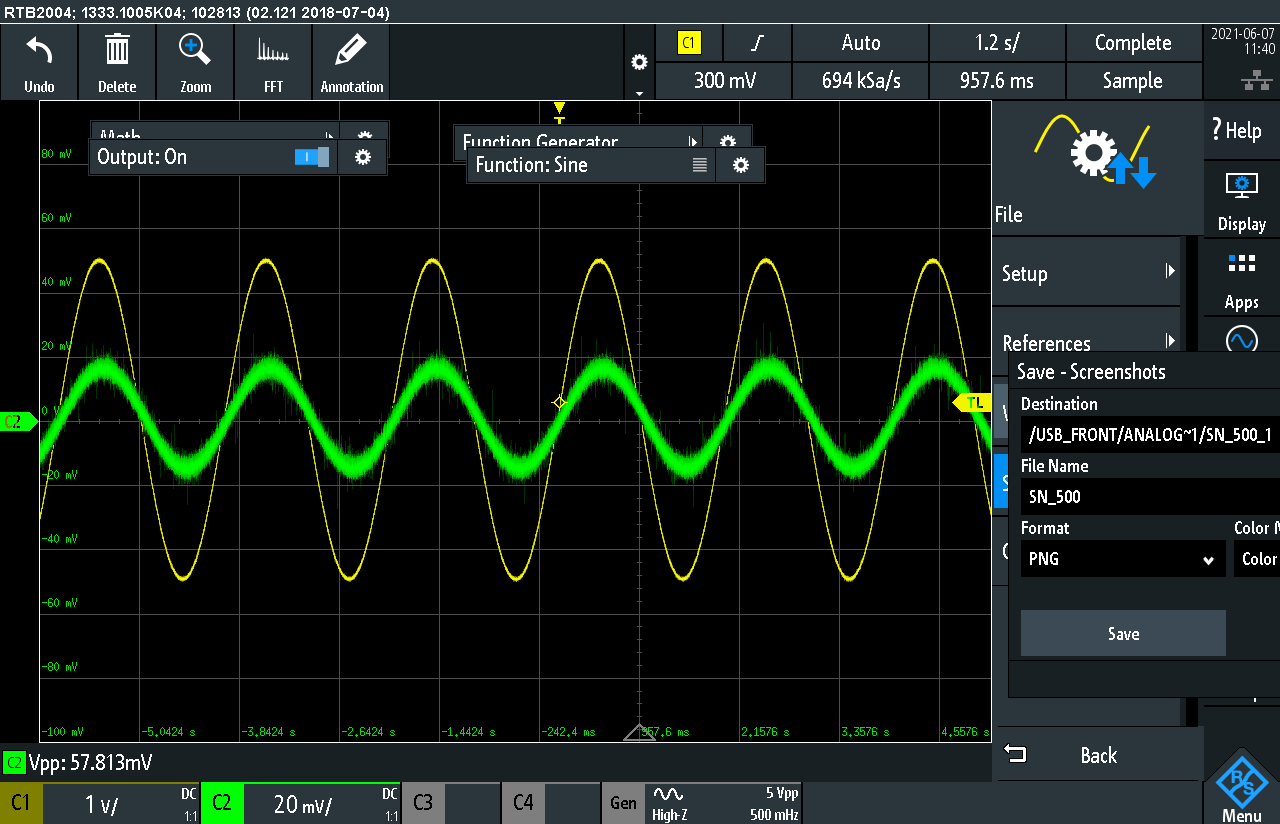
\includegraphics[scale = 0.10]{G2_N_500_pic.PNG}
            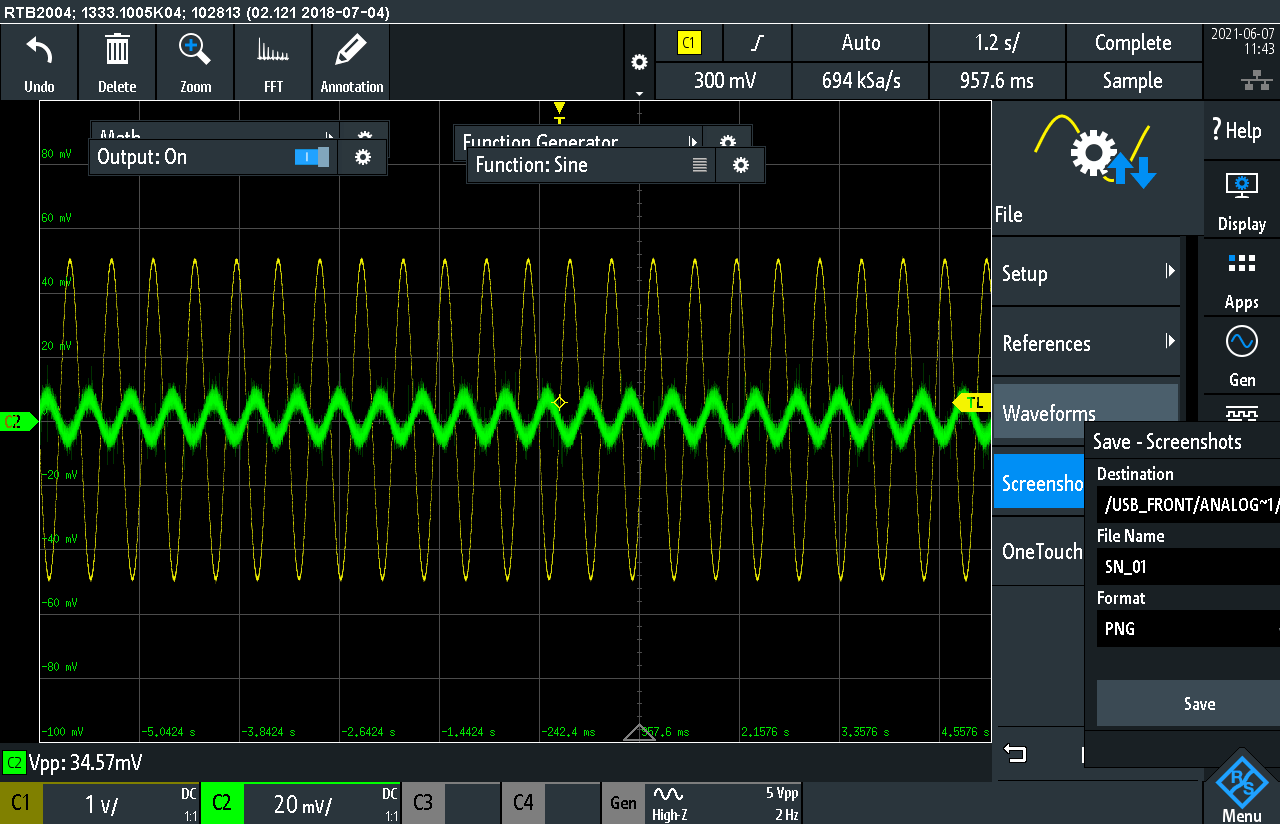
\includegraphics[scale = 0.10]{G2_N_2000_pic.PNG}
            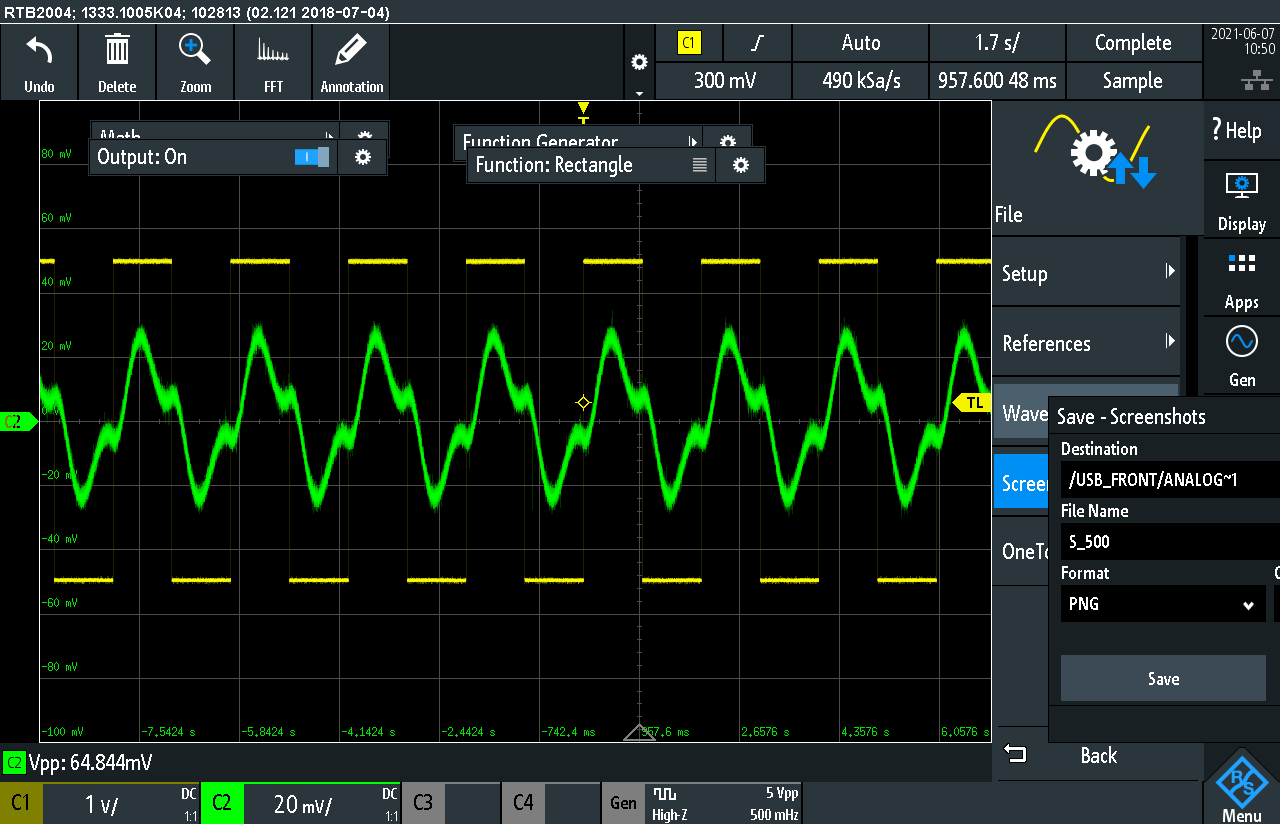
\includegraphics[scale = 0.10]{G2_S_500_pic.PNG}
            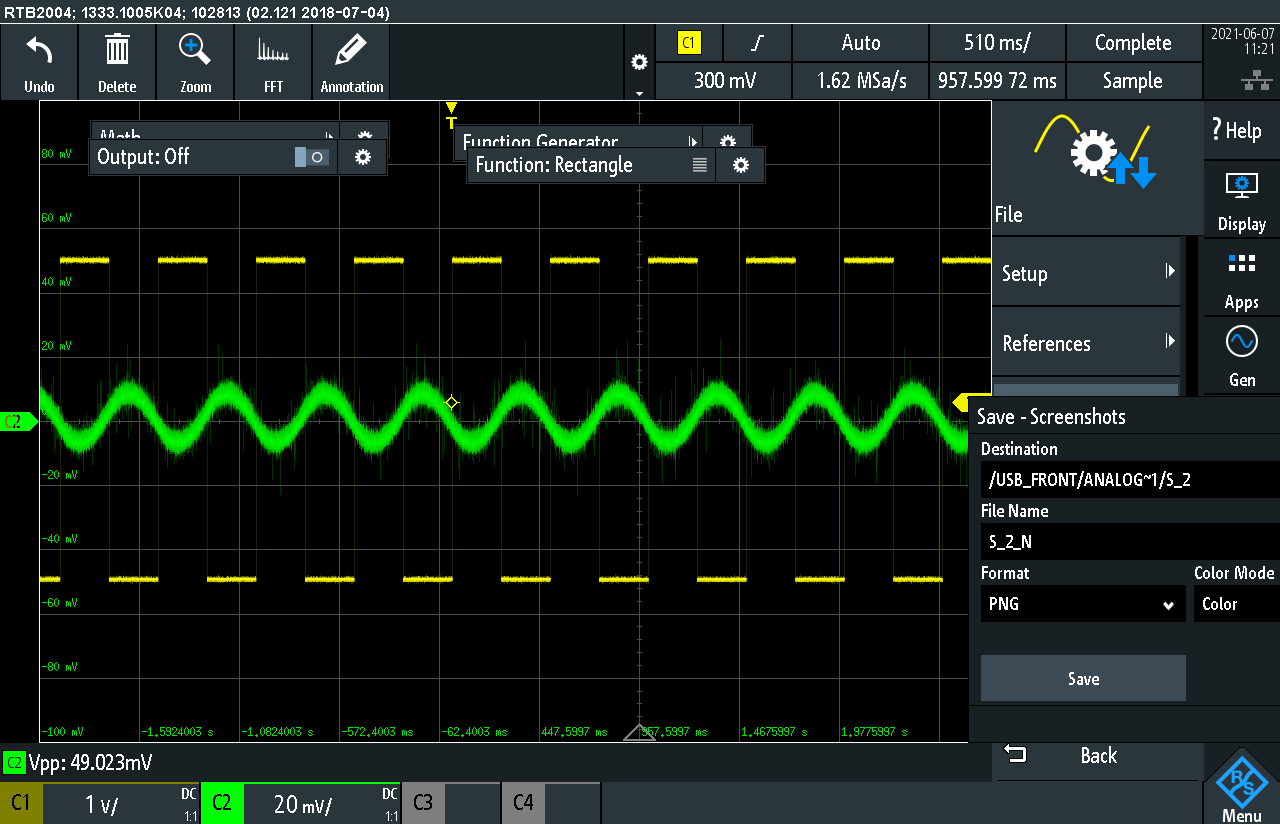
\includegraphics[scale = 0.10]{G2_S_2000_pic.PNG}
            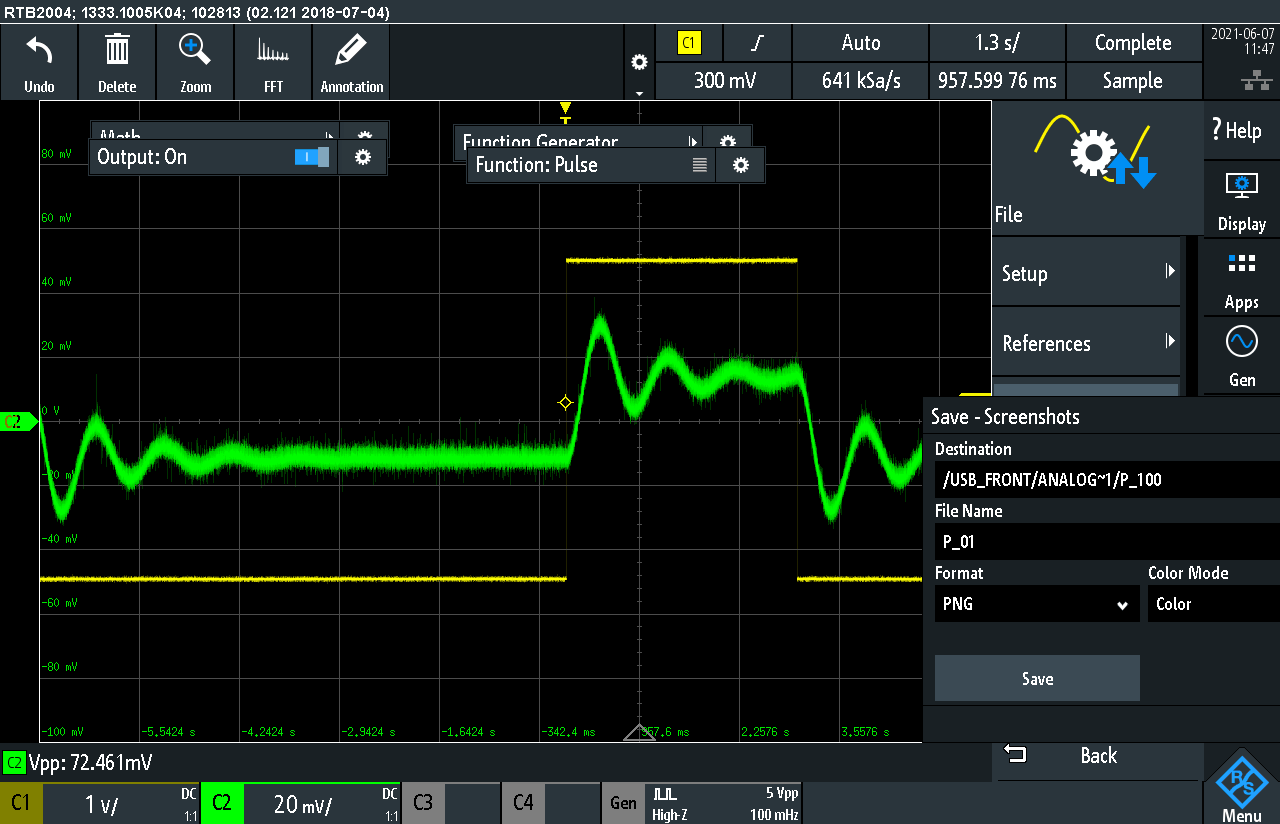
\includegraphics[scale = 0.10]{G2_P_100_pic.PNG}
            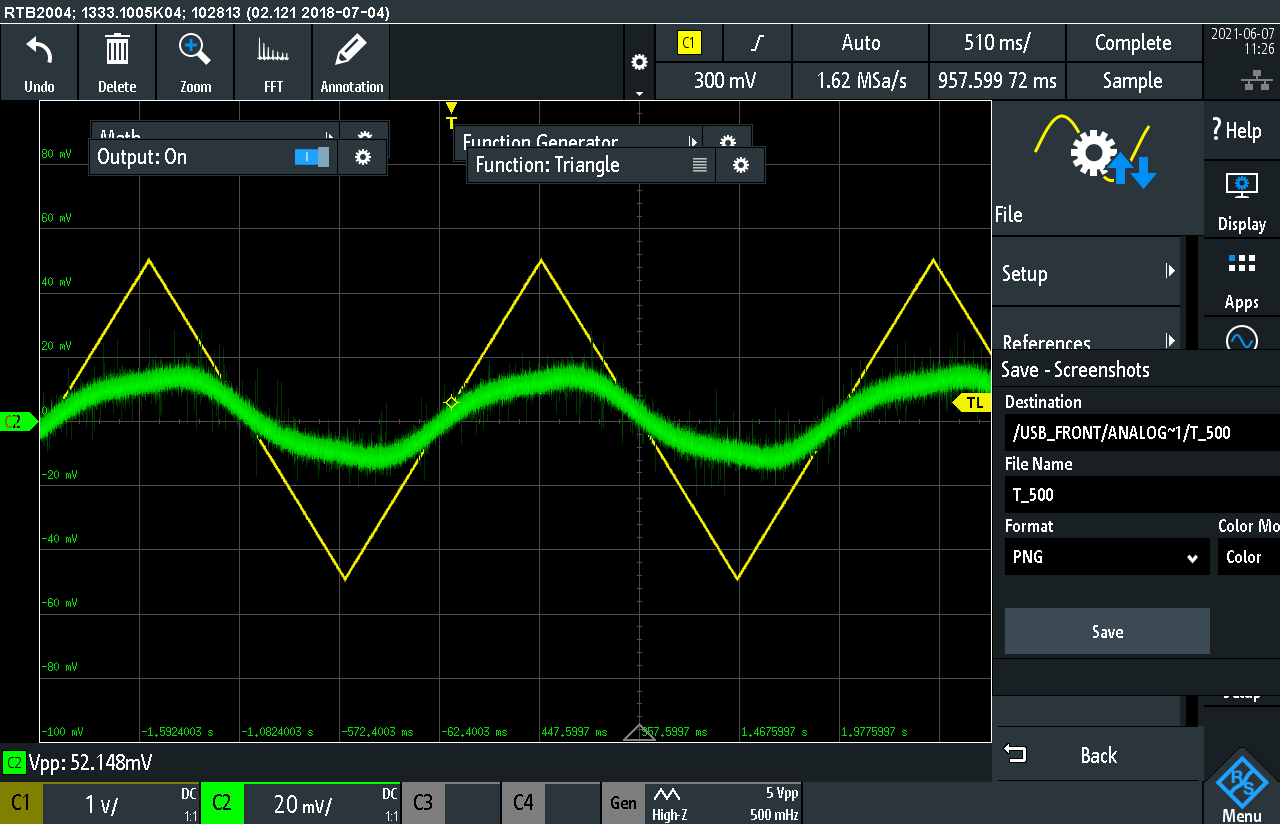
\includegraphics[scale = 0.10]{G2_T_500_pic.PNG}
            \caption{Standard Analogue Computer with $\gamma = 2$. Oscilloscope screenshots.}
        \end{figure}
        \begin{figure}[ht]
            
            \centering
            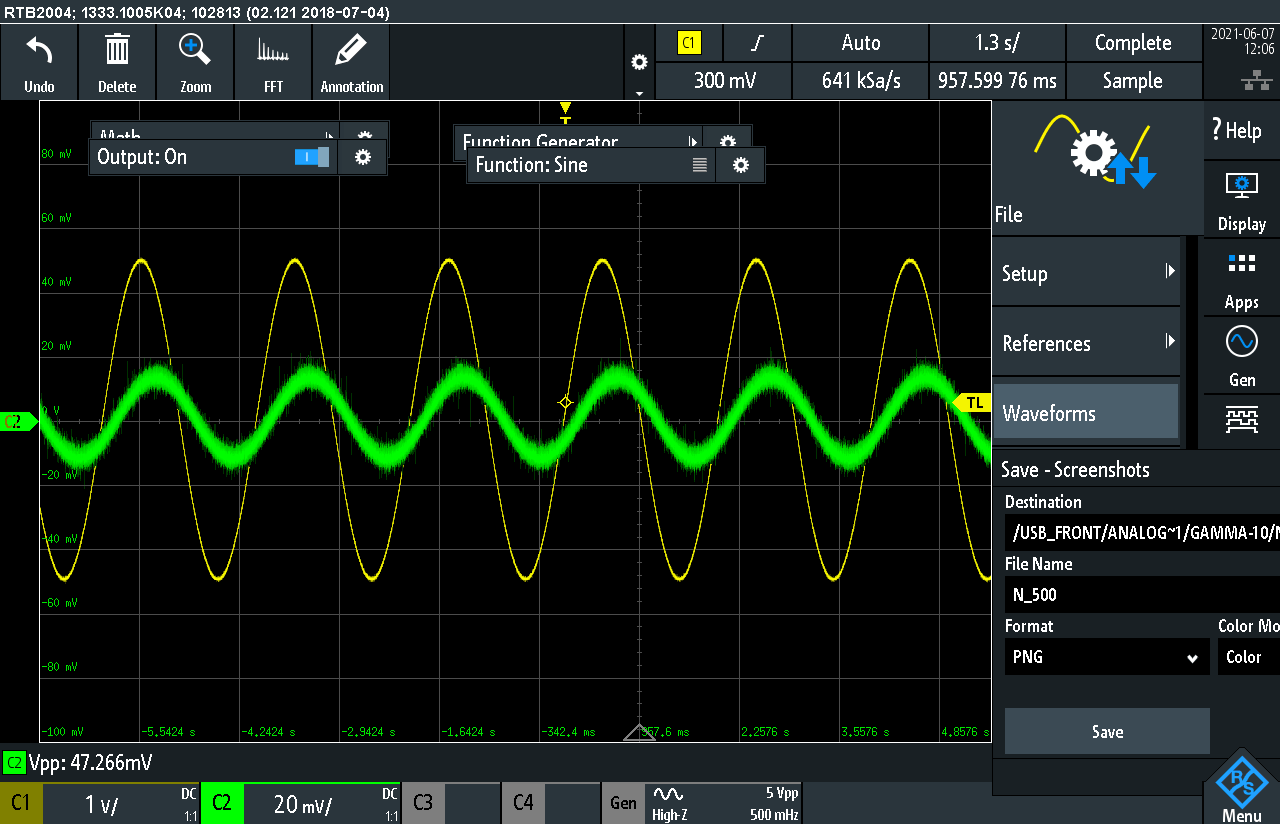
\includegraphics[scale = 0.10]{G10_N_500_pic.PNG}
            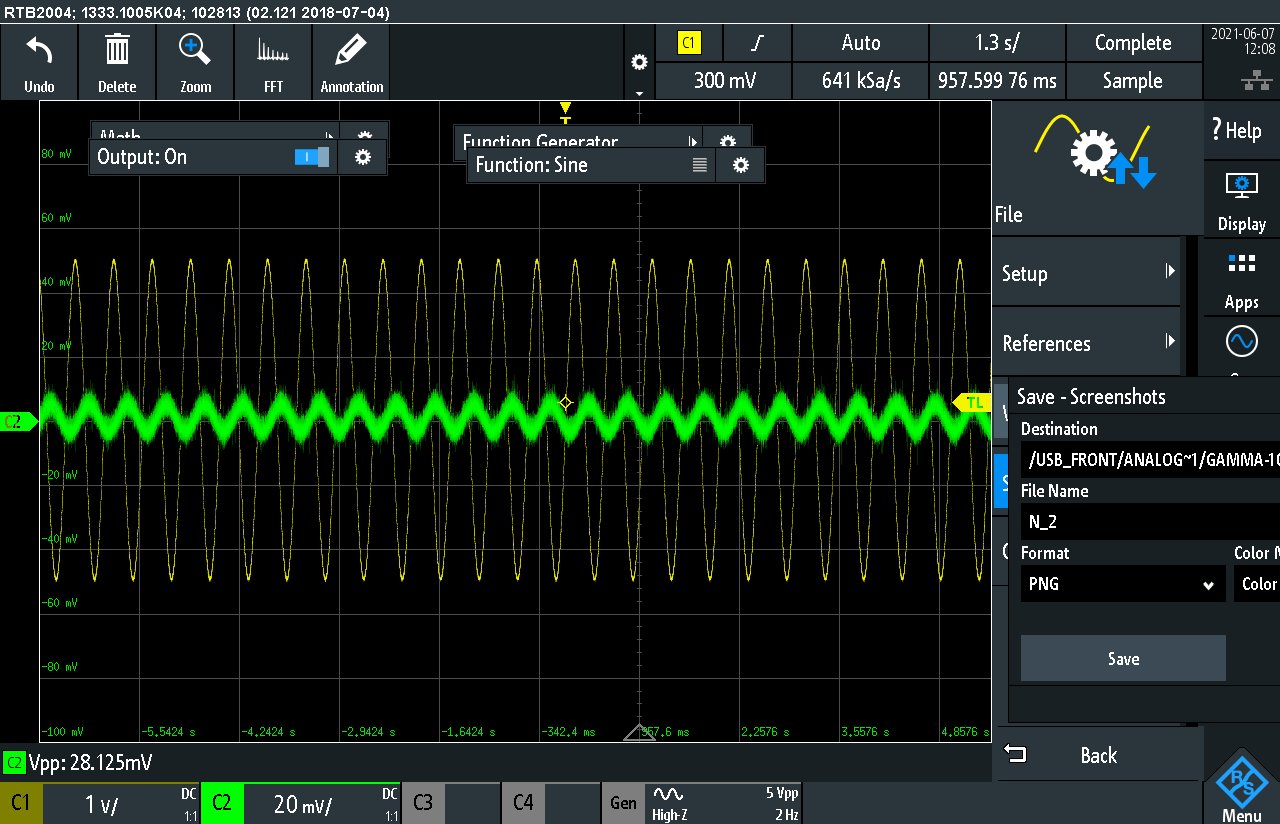
\includegraphics[scale = 0.10]{G10_N_2000_pic.PNG}
            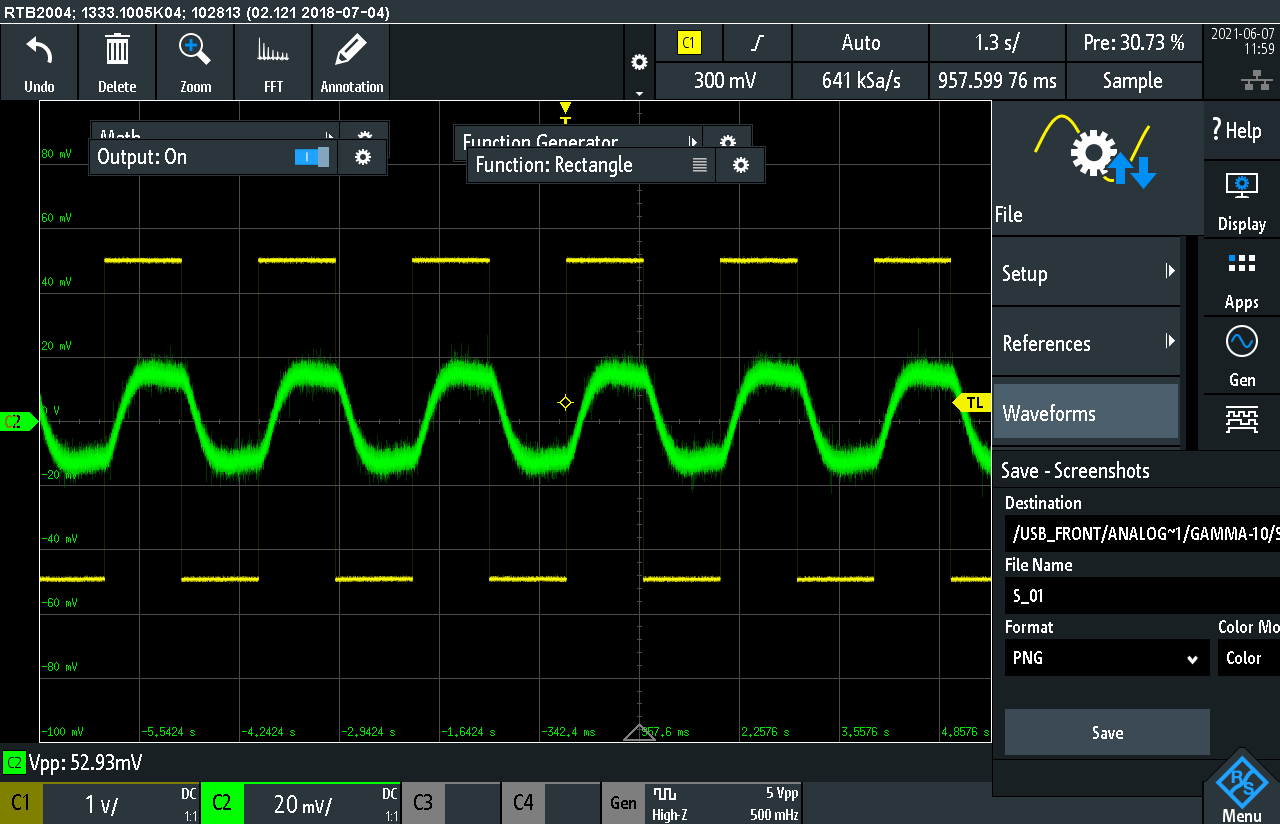
\includegraphics[scale = 0.10]{G10_S_500_pic.PNG}
            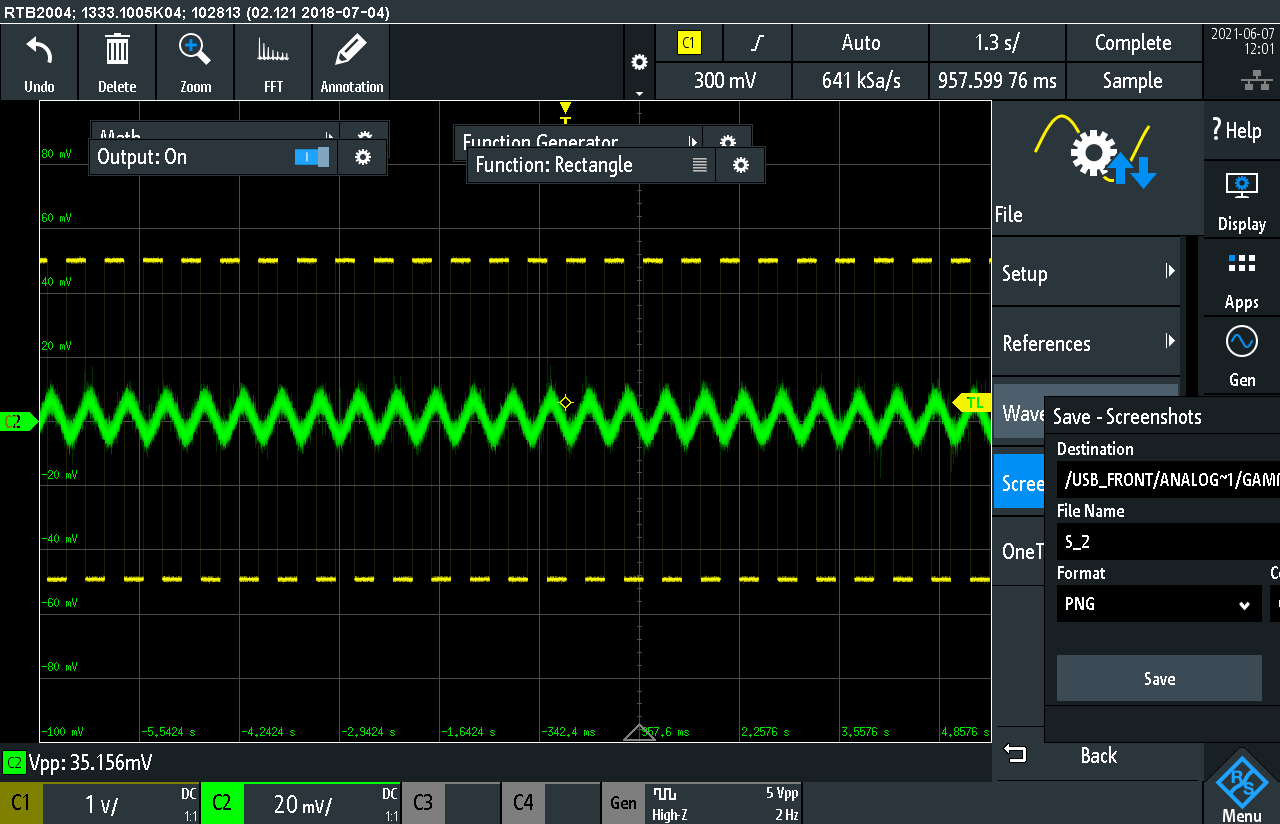
\includegraphics[scale = 0.10]{G10_S_2000_pic.PNG}
            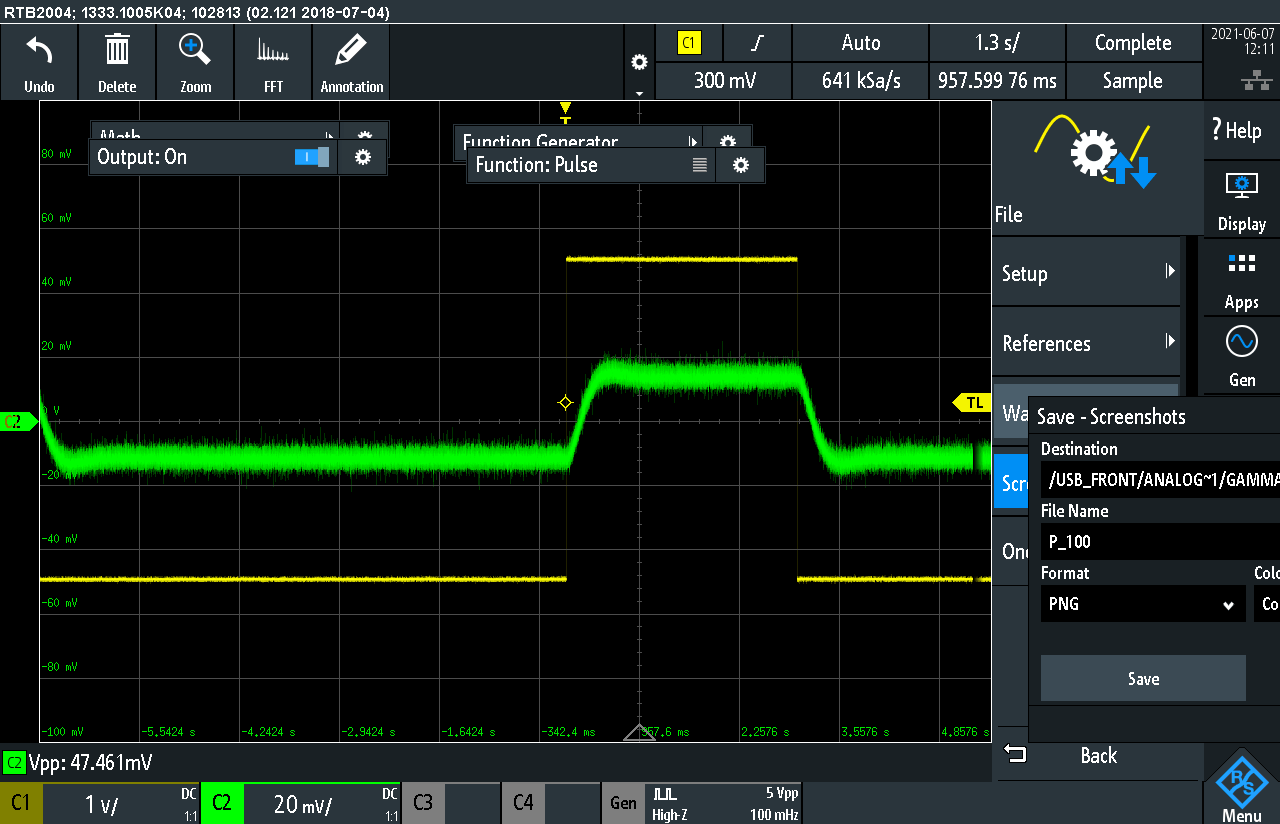
\includegraphics[scale = 0.10]{G10_P_100_pic.PNG}
            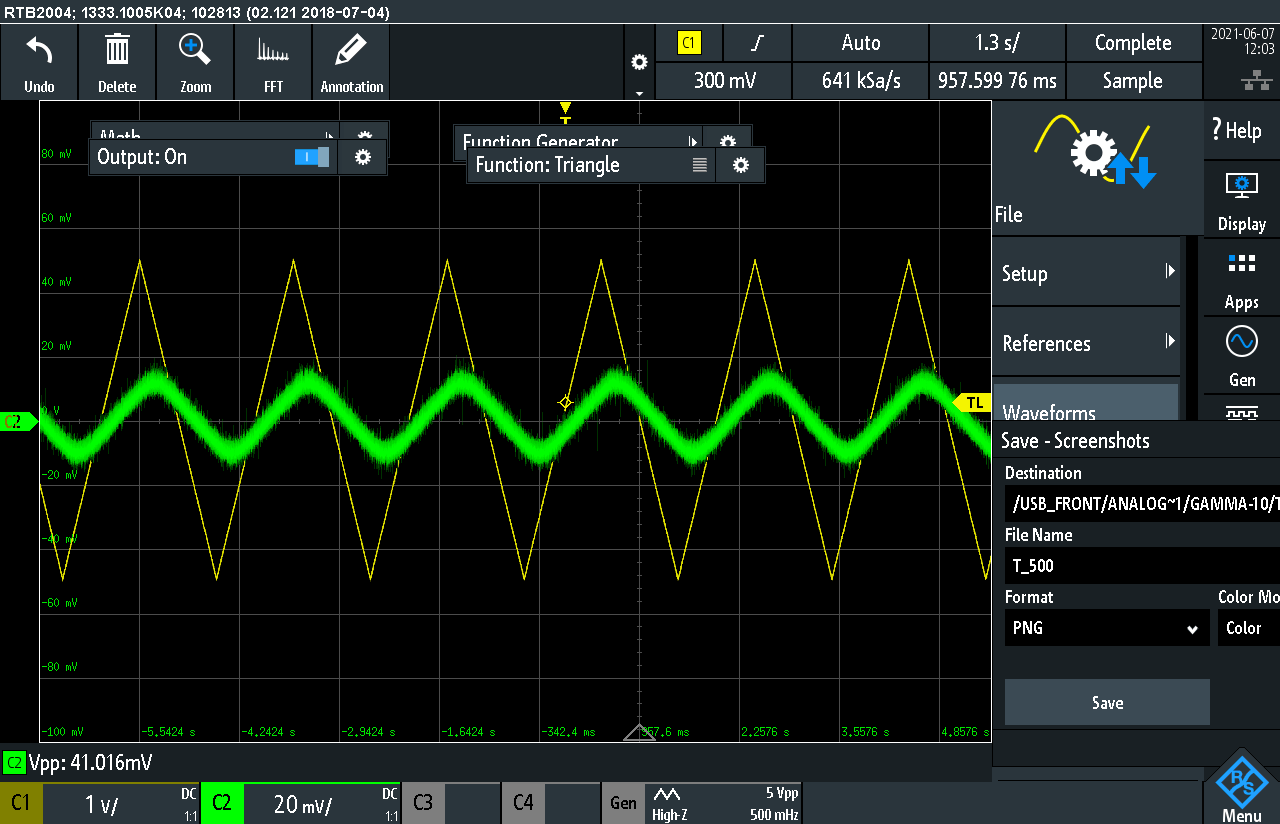
\includegraphics[scale = 0.10]{G10_T_500_pic.PNG}
            \caption{Standard Analogue Computer with $\gamma = 10$. Oscilloscope screenshots.}
        \end{figure}
        \clearpage
        \newpage
        \section{Moving Average and Fourier Data}
        \subsection{Moving Average}
        Moving average calculates the average representation of a given noisy signal via finite elemental analysis. For the given graphs, chucks of 200 datapoints were used as finite elements from the dataset of approximately 120000 datapoints for each graph. These were then ploted at the midpoint of the time range of each chunk.

        The error bands were calculated by using two moving averages of the maximum and minimum noise within each chunk. 

        \subsection{Fast Fourier Transform}

        Fast fourier transoform is an algorithm that computes the discrete Fourier Transform of a sequence of numbers.

        Time domain to frequency domain transformation is given by the equation:

        \begin{equation}
            \omega_k = \sum_{n = 0}^{N-1}t_n{e^{-i2\pi{\omega{n}}/N}} 
        \end{equation}

        
        \begin{figure}
            \label{G 2 Graphs}
            \centering
            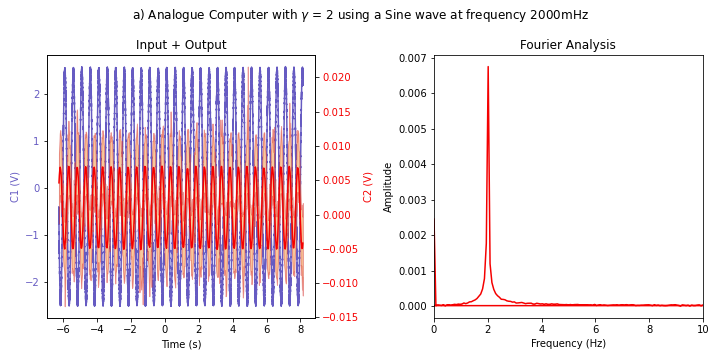
\includegraphics[scale = 0.30]{G 2 N_2000.png}
            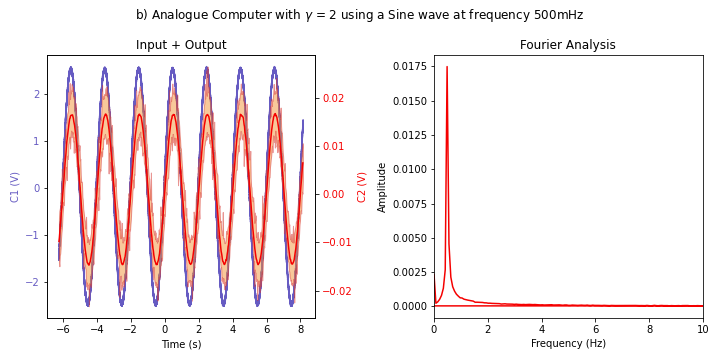
\includegraphics[scale = 0.30]{G 2 N_500.png}
            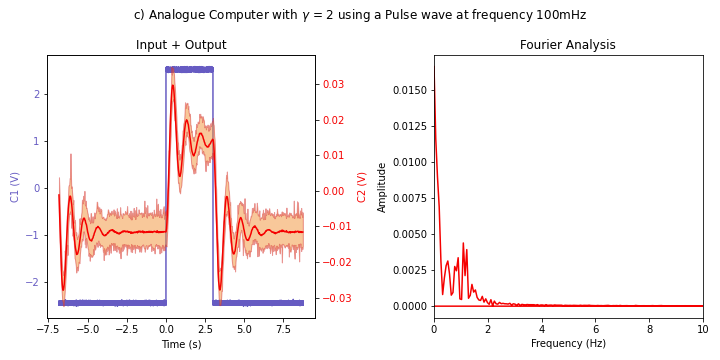
\includegraphics[scale = 0.30]{G 2 P_100.png}
            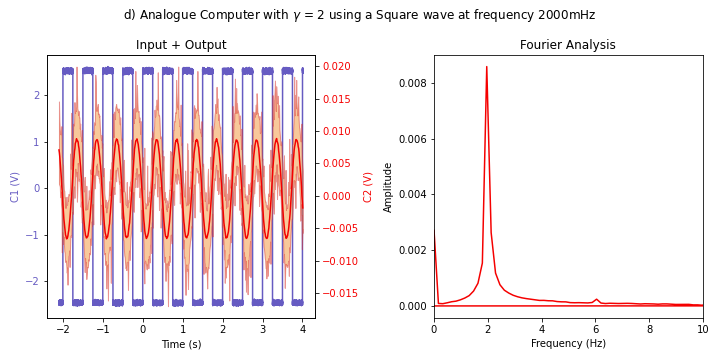
\includegraphics[scale = 0.30]{G 2 S_2000.png}
            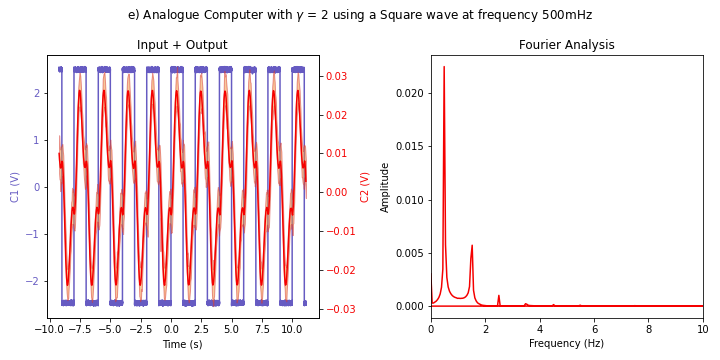
\includegraphics[scale = 0.30]{G 2 S_500.png}
            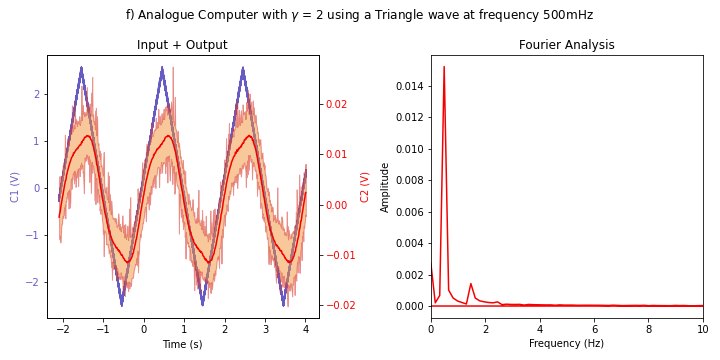
\includegraphics[scale = 0.30]{G 2 T_500.png}
            \caption{Standard Analogue Computer with $\gamma = 2$. Left hand side shows Input Wave (C1) and the moving average of the Output Wave (C2) with an error band. Right hand side shows the fourier transform from the time domain to the frequency domain of the C2 moving average.}
        \end{figure}
        \begin{figure}
            \label{G 10 Graphs}
            \centering
            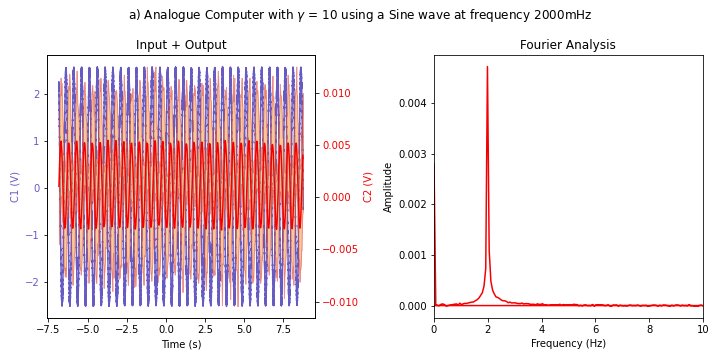
\includegraphics[scale = 0.30]{G 10 N_2000.png}
            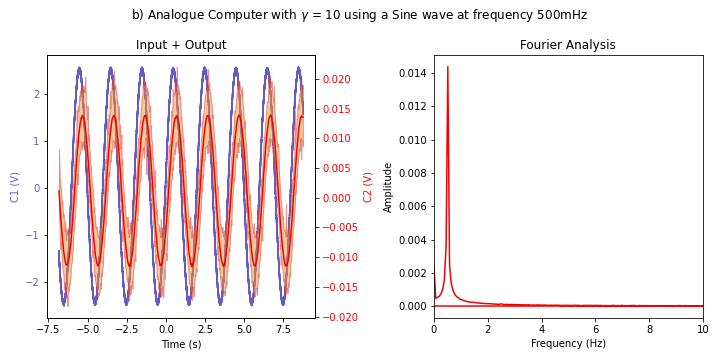
\includegraphics[scale = 0.30]{G 10 N_500.png}
            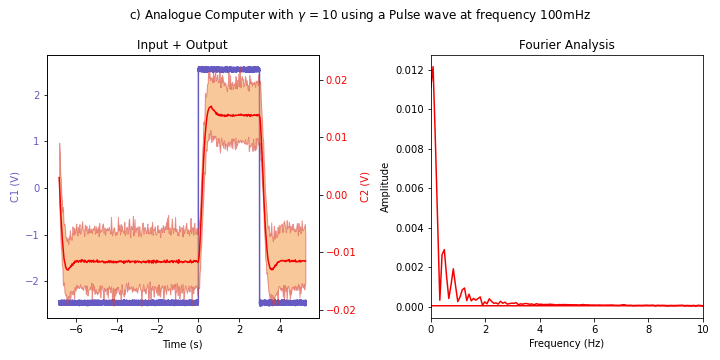
\includegraphics[scale = 0.30]{G 10 P_100.png}
            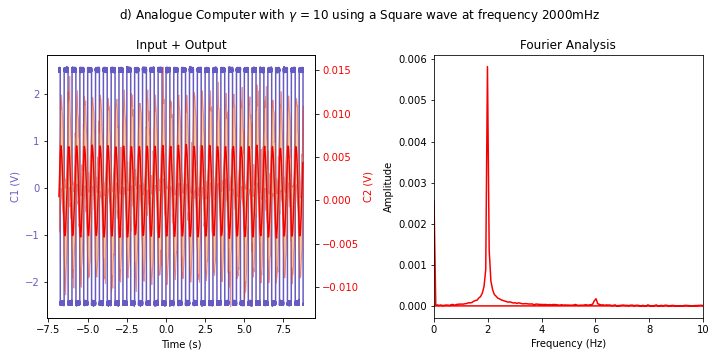
\includegraphics[scale = 0.30]{G 10 S_2000.png}
            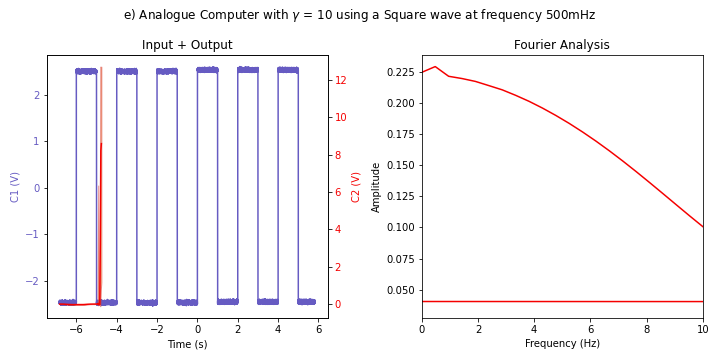
\includegraphics[scale = 0.30]{G 10 S_500.png}
            \caption{Standard Analogue Computer with $\gamma = 10$. Left hand side shows Input Wave (C1) and the moving average of the Output Wave (C2) with an error band. Right hand side shows the fourier transform from the time domain to the frequency domain of the C2 moving average. Figure e is quite anamolous, possibly due to corruption of data.}
        \end{figure}
        \begin{figure}
            \label{Inverted Diff G 2 Graphs}
            \centering
            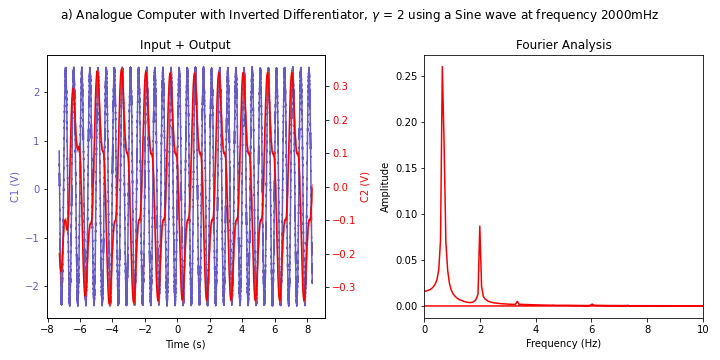
\includegraphics[scale = 0.30]{INVERTED DIFF G 2 N_2000.png}
            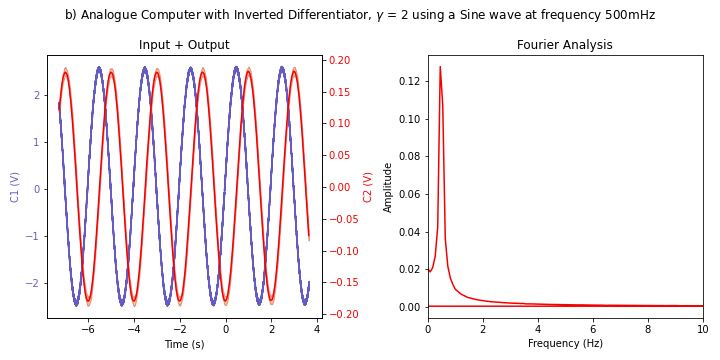
\includegraphics[scale = 0.30]{INVERTED DIFF G 2 N_500.png}
            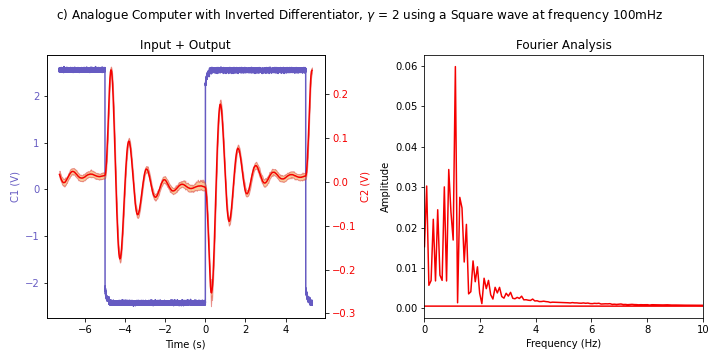
\includegraphics[scale = 0.30]{INVERTED DIFF G 2 S_100.png}
            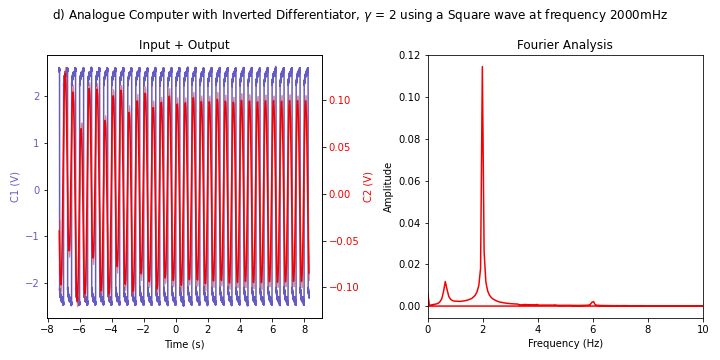
\includegraphics[scale = 0.30]{INVERTED DIFF G 2 S_2000.png}
            \caption{Analogue Computer with an Inverted Inverting Differentiator with $\gamma = 2$. Left hand side shows Input Wave (C1) and the moving average of the Output Wave (C2) with an error band. Right hand side shows the fourier transform from the time domain to the frequency domain of the C2 moving average.}
        \end{figure}
        \clearpage
    \end{appendices}
    \section{Acknowledgement}
    I would like thank my lab partner, Ari Alonso Bizzi for providing the diagrams and aiding with the experimetn. I would like to thank my lab instructor for aiding me with the experiment.
        
    \bibliographystyle{unsrt}
    \bibliography{ref}
\end{document}
